\documentclass{article}

\usepackage[a4paper, margin={2cm}, left={2.3cm}]{geometry}

\usepackage{graphicx}

\usepackage[ngerman]{babel}
\hyphenation{Software-entwicklung}

\usepackage[style=numeric,sorting=none]{biblatex}
\bibliography{bibliography.bib}

\usepackage[nottoc]{tocbibind}

\begin{document}
\title{\Large Einsendeaufgabe \\ Scrum}
\author{\normalsize Stefan Berger}
\date{}
\maketitle

\pagebreak

\tableofcontents

\pagebreak

\hspace{50px}

\begin{abstract}
Dieses Dokument beschreibt Projektmanagement mittels der Scrum-Technologie bzw. des Scrum-Frame\-works. Es gibt einen Überblick über die Entstehungsgeschichte von Scrum und die Personen, die an der Entwicklung beteiligt waren und sind. Es werden die wichtigsten Bestandteile von Scrum (Manifest für Agile Softwareentwicklung, Rollen der Teammitglieder und Artefakte) beschrieben und deren Nutzen erklärt. Im Fazit werden die drei Alleinstellungsmerkmale von Scrum – leichtgewichtig, leicht zu verstehen und schwer zu meistern – verdeutlicht.
\end{abstract}

\vspace{50px}

\raggedright\rightskip=0pt plus .2\hsize

\section{Einleitung}
\paragraph{}
Scrum ist ein Projektmanagement-Framework. Es existiert seit etwas mehr als zehn Jahren und ist aus Strategien hervorgegangen, die in Asien und den USA erfolgreich angewendet wurden. Im Unterschied zu anderen Projektmanagementstrategien akzeptiert es, dass Softwareentwicklungsprojekte unvorhersehbaren Änderungen unterliegen.

\paragraph{}
Im ersten Abschnitt werden wir uns mit der Entstehungsgeschichte von Scrum beschäftigen. Die Erfinder und Erhalter von Scrum hatten konkrete Vorstellungen, die mit Scrum verwirklicht und Problemstellungen, die gelöst werden. Im zweiten Abschnitt geht es um genau diese Personen und deren Beiträge zu Scrum. Im Manifest für Agile Softwareentwicklung sind die Grundregeln für den Erfolg bei der Anwendung von Scrum festgehalten, die im dritten Abschnitt behandelt werden. Der vierte Abschnitt beschäftigt sich mit den verschiedenen Rollen, die Scrum für die Teammitglieder vorsieht – Product Owner, Scrum Master und Entwickler. Im fünften Abschnitt beschäftigen wir uns mit den verschiedenen Artefakten des Frameworks.

\section{Geschichte}
\paragraph{}
Vor Scrum gab es bereits andere agile Projektmanagement-Ansätze. Elemente des Extreme Programming (XP) \cite{beck} fließen in das Scrum-Framework ein. XP ist ebenfalls leichtgewichtig und sieht die Entwicklung in Iterationen vor. Continuous Integration ist ein weiteres Konzept von XP, das oft zusammen mit Scrum angewendet wird. Das Manifest für Agile Softwareentwicklung bezeichnet kontinuierliche Auslieferung von Software als die höchste Priorität \cite{manifesto}.

\paragraph{}
Verschiedene andere Projektmanagement-Ansätze waren denen von Scrum sehr ähnlich. Hirotaka Takeuchi und Ikujiro Nonaka verglichen als erstes den Prozess mit Rugby \cite[S.~1]{takeuchi}. Wie in dem Sport der Ball zwischen den Spielern hin- und hergeworfen wird, um das Team vorwärts zu bewegen, sollen sich die Projektteammitglieder gegenseitig zuarbeiten, um das Projekt voranzubringen. Einige Charakteristika des Ansatzes finden sich in Scrum wieder, etwa die „eingebaute Instabilität“ und selbstorganisierte Projektteams \cite[S.~4]{takeuchi}.

\paragraph{}
James O. Coplien berichtet in \glqq Borland Software Craftsmanship: A New Look at Process, Quality and Productivity\grqq{} von einem Projekt bei Borland, in dem den Teammmitgliedern auf kreative Weise Rollen zugewiesen wurden \cite[S.~3]{coplien}. Es wurde großen Wert auf Meetings gelegt, und es konnte schnell auf Änderungen an der Architektur reagiert werden \cite[S.~7]{coplien}.

\paragraph{}
1997 veröffentlichte Ken Schwaber das Paper „SCRUM Development Process“ \cite{schwaber}. Das Manifest für Agile Softwareentwicklung wurde 2001 von zunächst 17 Personen unterschrieben, unter anderem von Ken Schwaber, Jeff Sutherland und Mike Beedle. 2002 folgte das Buch \glqq Agile Software Development With Scrum\grqq{}, von Ken Schwaber und Mike Beedle.

\pagebreak

\section{Personen}
\subsection{Ken Schwaber}
\paragraph{}
Ken Schwaber hat den Scrum-Prozess zusammen mit Jeff Sutherland in den frühen 1990er Jahren mitenwickelt, um Organisationen bei der Bewältigung komplexer Entwicklungsprojekte zu helfen. Als einer der Unterzeichner des Manifests für Agile Softwareentwicklung in 2001 gründete er anschließend die Agile Alliance und die Scrum Alliance. Die Scrum Alliance verließ er kürzlich, um Scrum.org zu gründen.

\paragraph{}
Ken Schwaber hat 30 Jahre Erfahrung in der Softwareindustrie und hat drei Bücher über Scrum geschrieben: \glqq Agile Software Development with Scrum\grqq{}, \glqq Agile Project Management with Scrum\grqq{} und \glqq The Enterprise and Scrum\grqq{}. Er lebt in Lexington, Massachusetts. (\cite{ken}, Übersetzung des Autors)

\begin{figure}[h]
  \centering
  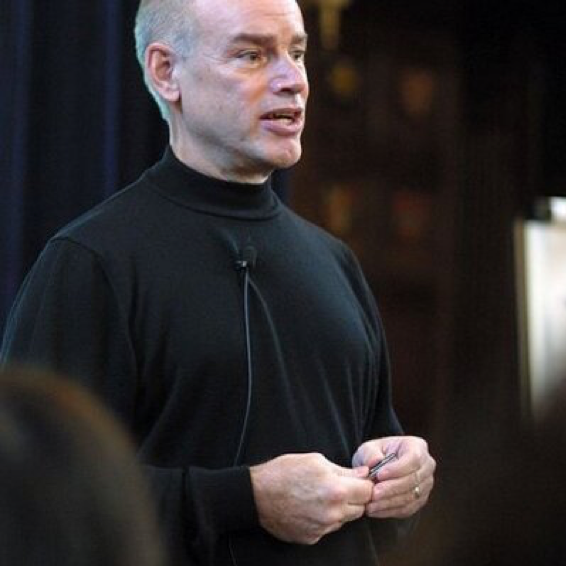
\includegraphics[scale=.45]{img/ken.png}
  \caption{Ken Schwaber}
  \label{kenpng}
\end{figure}

\subsection{Jeff Sutherland}
\paragraph{}
Jeff Sutherland ist Mitgestalter von Scrum und ein führender Experte auf dem Gebiet der Entwicklung des Frameworks, um die Anforderungen heutiger Unternehmen zu erfüllen. Die Methodik, die er 1993 entwickelte und 1995 mit Ken Schwaber formalisierte, wurde seitdem von der überwiegenden Mehrheit der weltweiten Softwareentwicklungsunternehmen eingeführt. Aber Jeff Sutherland erkannte, dass die Vorteile von Scrum nicht auf Software- und Produktentwicklung beschränkt sind. Er passte diese erfolgreiche Strategie für mehrere andere Industrien an, einschließlich der Finanz-, Gesundheits-, Bildungs- und Telekommunikationsindustrie.

\paragraph{}
Als Geschäftsführer von Scrum Inc. und Senior Advisor und Agile Coach für OpenView Venture Partners erstellt Jeff Sutherland die Vision für Erfolg mit Scrum. Er teilt weiterhin Best Practices mit Organisationen auf der ganzen Welt und hat ausführlich über Scrum-Regeln und -Methoden geschrieben. Mit einem tiefen Verständnis von Geschäftsprozessen – gesammelt in den Jahren als CTO/CEO von elf verschiedenen Softwarebetrieben – besitzt Jeff Sutherland die Fähigkeit zu beschreiben, was die Vorteile von Scrum auf hoher organisatorischer Ebene sind und was es braucht, um hyperproduktive Teams zu erstellen. (\cite{jeff},~Übersetzung~des~Autors)

\begin{figure}[h]
  \centering
  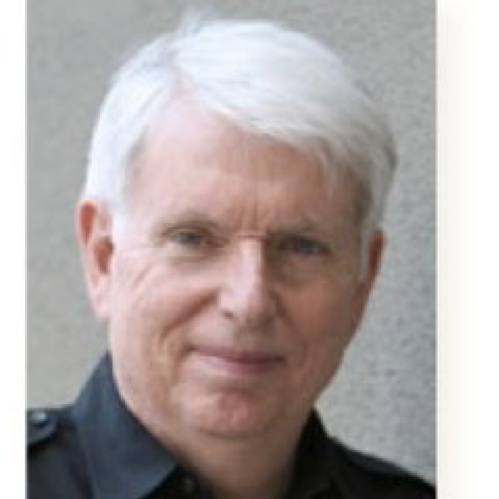
\includegraphics[scale=.5]{img/jeff.png}
  \caption{Jeff Sutherland}
  \label{jeffpng}
\end{figure}

\pagebreak

\subsection{Hirotaka Takeuchi}
\paragraph{}
Hirotaka Takeuchi war Assistant Professor an der Harvard Business School von 1976 bis 1983, wo er im M.B.A.-Programm Kurse in Marketing und Einzelhandel gab. Er fing 1983 als Associate Professor an der Hitotsubashi Universität Tokyo an und wurde 1987 Professor. 1989 und 1990 war er als Gastprofessor wieder an der Harvard Business School und lehrte dort „Konkurrenz und Strategie“. (\cite{hiro}, Übersetzung des Autors)

\begin{figure}[h]
  \centering
  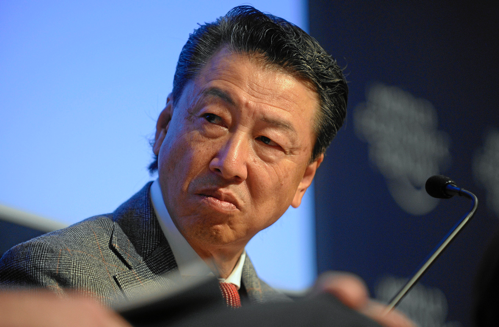
\includegraphics[scale=.85]{img/hiro.png}
  \caption{Hirotaka Takeuchi}
  \label{hiropng}
\end{figure}


\subsection{Ikujirō Nonaka}
\paragraph{}
Ikujirō Nonaka erhielt 1958 seinen BA in Politikwissenschaften von der Waseda-Universität und 1968 bzw. 1972 den MBA und den Doktortitel in Business Administration von der University of California, Berkeley.
[\ldots]
\paragraph{}
Professor Nonakas vorwiegendes Forschungsinteresse ist es, die Theorie des wissensbasierten Managements von Unternehemen, Gemeinschaften, öffentlicher Verwaltung und Nationen zu begründen und zu verbreiten, um die laufende, nachhaltige Wissensschöpfung und Innovation zu fördern. Als Teil seiner Arbeit hat er vergleichende Forschung mit Führungskräften und an wissensschöpfenden Prozessen in Unternehmen und Organisationen und von Führungskräften auf der ganzen Welt durchgeführt.
[\ldots]
\paragraph{}
\glqq The Knowledge-Creating Company\grqq{} und \glqq Enabling Knowledge Creation\grqq{} erhielten 1996 beziehungsweise 2000 den \glqq Best Book of the Year\grqq{} award in Business und Management von der Association of American Publishers, Inc. (\cite{ikuji}, Übersetzung des Autors)

\begin{figure}[h]
  \centering
  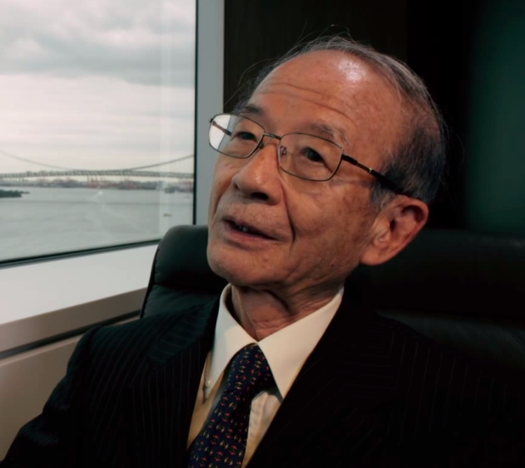
\includegraphics[scale=.7]{img/ikuji.png}
  \caption{Ikujirō Nonaka}
  \label{ikujipng}
\end{figure}

\pagebreak

\subsection{Kent Beck}
\paragraph{}
Kent Beck, einer der kreativsten und meistgefeierten Führungspersonen der Softwareindustrie, stellt konsequent Softwaretechnik-Dogmas infrage und treibt Ideen wie Muster, Test-Driven-Development und Extreme-Programming voran. Er gehört derzeit dem Three Rivers Institute und Agitar Software an und ist der Autor vieler Addison-Wesley-Titel, einschließlich „Test-Driven Development“ (2003) und, mit Cynthia Andres, „Extreme Programming Explained, Second Edition“ (2005). \\
(\cite[Buchrückseite]{beck2},~Übersetzung~des~Autors)

\begin{figure}[h]
  \centering
  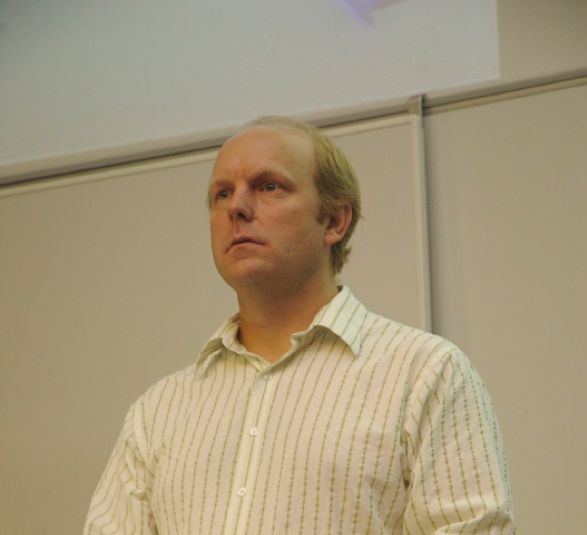
\includegraphics[scale=.75]{img/kent.png}
  \caption{Kent Beck}
  \label{kentpng}
\end{figure}

\subsection{Mike Beedle}
\paragraph{}
Mike Beedle war der zweite frühzeitige Scrum-Anwender nach Jeff Sutherland’s Scrum-Team in Boston, mit Erfahrung im Praktizieren von Scrum seit Mitte 1995 in einer Vielzahl von Geschäftsumfeldern.

\paragraph{}
Mike Beedle und seine Unternehmen haben Scrum, Enterprise Scrum und Business Agility bei zigtausenden Menschen und tausenden Unternehmen eingeführt und bieten Training, Consulting, Mentoring und Coaching an.
[\ldots] (\cite[Buchrückseite]{beck2},~Übersetzung~des~Autors)

\begin{figure}[h]
  \centering
  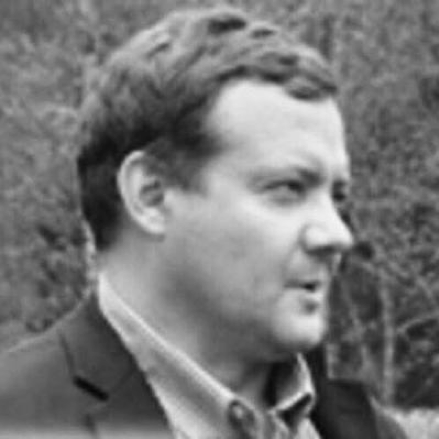
\includegraphics[scale=.85]{img/mike.png}
  \caption{Mike Beedle}
  \label{mikepng}
\end{figure}

\pagebreak

\section{Manifest für Agile Softwareentwicklung}
\paragraph{}
Das Manifest für Agile Softwareentwicklung beschreibt zuerst 4 Prioritäten der Wertschätzung bei der Softwareentwicklung:
\vspace{10px}

{
\centering
\textit{Individuen und Interaktionen mehr als Prozesse und Werkzeuge}

\textit{Funktionierende Software mehr als umfassende Dokumentation}

\textit{Zusammenarbeit mit dem Kunden mehr als Vertragsverhandlung}

\textit{Reagieren auf Veränderung mehr als das Befolgen eines Plans}

}
\paragraph{}
Es legt weiterhin zwölf Prinzipien fest:

{
\centering
\paragraph{}
\textit{Unsere höchste Priorität ist es, den Kunden durch frühe und kontinuierliche Auslieferung wertvoller Software zufrieden zu stellen.}

\paragraph{}
\textit{Heisse Anforderungsänderungen selbst spät in der Entwicklung willkommen. Agile Prozesse nutzen Veränderungen zum Wettbewerbsvorteil des Kunden.}

\paragraph{}
\textit{Liefere funktionierende Software regelmäßig innerhalb weniger Wochen oder Monate und bevorzuge dabei die kürzere Zeitspanne.}

\paragraph{}
\textit{Fachexperten und Entwickler müssen während des Projektes täglich zusammenarbeiten.}

\paragraph{}
\textit{Errichte Projekte rund um motivierte Individuen. Gib ihnen das Umfeld und die Unterstützung, die sie benötigen und vertraue darauf, dass sie die Aufgabe erledigen.}

\paragraph{}
\textit{Die effizienteste und effektivste Methode, Informationen an und innerhalb eines Entwicklungsteams zu übermitteln, ist im Gespräch von Angesicht zu Angesicht.}

\paragraph{}
\textit{Funktionierende Software ist das wichtigste Fortschrittsmaß.}

\paragraph{}
\textit{Agile Prozesse fördern nachhaltige Entwicklung. Die Auftraggeber, Entwickler und Benutzer sollten ein gleichmäßiges Tempo auf unbegrenzte Zeit halten können.}

\paragraph{}
\textit{Ständiges Augenmerk auf technische Exzellenz und gutes Design fördert Agilität.}

\paragraph{}
\textit{Einfachheit -- die Kunst, die Menge nicht getaner Arbeit zu maximieren -- ist essenziell.}

\paragraph{}
\textit{Die besten Architekturen, Anforderungen und Entwürfe entstehen durch selbstorganisierte Teams.}

\paragraph{}
\textit{In regelmäßigen Abständen reflektiert das Team, wie es effektiver werden kann und passt sein Verhalten entsprechend an.}

}
\cite{manifesto}

\section{Rollen}
\subsection{Product Owner}
\paragraph{}
Der Product Owner ist dafür verantwortlich, den Wert des Produktes zu maximieren, das aus der Arbeit des Entwicklungsteams entsteht. Wie dies geschieht, kann je nach Organisation, Scrum-Team und Einzelpersonen stark variieren. Der Product Owner ist die einzige Person, die für das Management des Product Backlogs verantwortlich ist. Das Product-Backlog-Management umfasst:
\begin{itemize}
\item{die Product-Backlog-Einträge klar zu formulieren;}
\item{die Einträge im Product Backlog so zu sortieren, dass Ziele und Missionen optimal erreicht werden können;}
\item{den Wert der Arbeit zu optimieren, die das Entwicklungsteam erledigt;}
\item{sicherzustellen, dass das Product Backlog sichtbar, transparent und für alle klar ist sowie zeigt, woran das Scrum-Team als nächstes arbeiten wird; und}
\item{sicherzustellen, dass das Entwicklungsteam die Product-Backlog-Einträge im erforderlichen Maße versteht.}
\end{itemize}

\paragraph{}
Der Product Owner kann die oben genannten Arbeiten selbst durchführen oder sie durch das Entwicklungsteam erledigen lassen. Der Product Owner bleibt jedoch immer rechenschaftspflichtig.
\cite[S.~6]{scrum}

\subsection{Entwicklungsteam}
\paragraph{}
Das Entwicklungsteam besteht aus Profis, die am Ende eines jeden Sprints ein fertiges [„Done“] Inkrement übergeben, welches potenziell auslieferbar ist. Im Sprint Review muss ein fertiges Inkrement vorhanden sein. Nur Mitglieder der Entwicklungsteams erstellen das Produktinkrement.

\paragraph{}
Entwicklungsteams sind von der Organisation so strukturiert und befähigt, dass sie ihre eigene Arbeit selbst organisieren und managen. Die daraus resultierende Synergie optimiert die Gesamteffizienz und -Effektivität des Entwicklungsteams.
\cite[S.~7]{scrum}

\subsection{Scrum Master}
\paragraph{}
Der Scrum Master ist dafür verantwortlich, Scrum entsprechend des Scrum Guides zu fördern und zu unterstützen. Scrum Master tun dies, indem sie allen Beteiligten helfen, die Scrum- Theorie, Praktiken, Regeln und Werte zu verstehen.

\paragraph{}
Der Scrum Master ist ein „Servant Leader“ für das Scrum-Team. Der Scrum Master hilft denjenigen, die kein Teil des Scrum-Teams sind, zu verstehen, welche ihrer Interaktionen mit dem Team sich hilfreich auswirken und welche nicht. Der Scrum Master hilft dabei, die Zusammenarbeit so zu optimieren, dass der durch das Scrum-Team generierte Wert maximiert wird.
\cite[S.~8]{scrum}

\section{Artefakte}
\subsection{Product Backlog}
Das Product Backlog ist eine geordnete Liste von allem, von dem bekannt ist, dass es im Produkt enthalten sein soll. Es dient als einzige Anforderungsquelle für alle Änderungen am Produkt. Der Product Owner ist für das Product Backlog, seine Inhalte, den Zugriff darauf und die Reihenfolge der Einträge verantwortlich.
\cite[S.~15]{scrum}

\subsection{Sprint Backlog}
\paragraph{}
Das Sprint Backlog ist die Menge der für den Sprint ausgewählten
Product-Backlog-Einträge, ergänzt um einen Plan, um das Produktinkrement zu liefern und das Sprint-Ziel zu erreichen. Das Sprint Backlog ist eine Prognose des Entwicklungsteams darüber, welch e Funktionalität im nächsten Inkrement enthalten sein wird, sowie über die erforderliche Arbeit, um diese Funktionalität in einem fertigen [„Done“] Inkrement zu liefern.
\cite[S.~16]{scrum}

\subsection{Inkrement}
\paragraph{}
Das Inkrement ist das Ergebnis aus allen in einem Sprint fertiggestellten Product-Backlog-Einträge n und dem Resultat der Inkremente aller früheren Sprints. Am Ende eines Sprints muss das neue Inkrement fertig ["Done"] sein; das heißt es muss in einem verwendbaren Zustand sein und die Definition of Done des Teams erfüllen. Ein Inkrement ist ein Gegenstand inspizierbarer, fertiger [„Done“] Arbeit, der die Empirie am Ende des Sprints unterstützt. Das Inkrement ist ein Schritt in Richtung einer Vision oder eines Ziels. Es muss auch dann im einsatzfähigen Zustand sein, wenn der Product Owner es aktuell noch gar nicht ausliefern will.
\cite[S.~17]{scrum}

\section{Fazit}
\paragraph{}
Scrum ist leichtgewichtig, denn es unterteilt den Prozess der Softwareentwicklung in Iterationen, und das Team plant nur eine Iteration genau voraus. Die Planungen der nächsten Iterationen basieren dann in einem erheblichen Maß auf den Ergebnissen der vorherigen.

\paragraph{}
Scrum ist außerdem leicht zu verstehen. Das liegt zum einen an der Leichtgewichtigkeit und zum anderen daran, dass keine Vorkenntnisse des Projektmanagements notwendig sind, um die Konzepte zu verstehen und auszuprobieren. Zwar ist es am Anfang vor allem für Softwareentwickler ungewohnt, aber leicht anzuwenden.

\paragraph{}
Schließlich ist Scrum schwer zu meistern. Es erfordert viel Übung, die Artefakte des Frameworks so anzuwenden, dass die bestmögliche Software oder Software, die gut genug ist \cite{bach} entwickelt werden kann.

\pagebreak

\printbibliography[heading=bibintoc,title=Literaturverzeichnis]

\pagebreak

\listoffigures

\end{document}
